% 2017 全国Ⅰ卷 理7：多面体三视图
% 正视图/左视图 = 边长 2 的正方形上叠等腰直角三角形；俯视图 = 等腰直角三角形
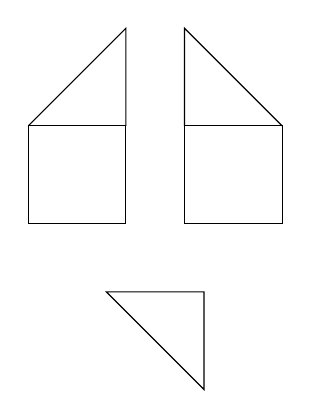
\begin{tikzpicture}[scale=0.62, font=\small]
  % 正视图（三角形直角边在右）
  \begin{scope}
    \draw (0,0) rectangle (2,2);
    \draw (0,2) -- (2,4) -- (2,2);
  \end{scope}
  % 左视图（三角形直角边在左）
  \begin{scope}[xshift=3.2cm]
    \draw (0,0) rectangle (2,2);
    \draw (0,2) -- (0,4) -- (2,2);
  \end{scope}
  % 俯视图（等腰直角三角形，直角边 2）
  \begin{scope}[yshift=-3.4cm, xshift=1.6cm]
    \draw (0,2) -- (2,2) -- (2,0) -- cycle;
  \end{scope}
\end{tikzpicture}
